\subsubsection{Qualitative evaluation on brain tumor resection dataset}

We used the \ac{BITE} dataset \cite{mercier_online_2012} to evaluate the ability of our self-supervised model to segment \acp{RC} on images from a different institution, modality and pathology than the datasets used for quantitative evaluation.
For postprocessing, all but the largest binary connected component were removed.
The model successfully segmented the \ac{RC} on 11/13 images, even though some contained challenging features (\cref{fig:bite}).

\newcommand{\qualit}[1]{\includegraphics[width=0.14\linewidth]{bite/cropped/#1}}
\newcommand{\qualitfig}[1]{
  \centering
  \qualit{#1_sag}%
  \enskip
  \qualit{#1_seg_sag}%
  \quad
  \qualit{#1_cor}%
  \enskip
  \qualit{#1_seg_cor}%
  \quad
  \qualit{#1_axi}%
  \enskip
  \qualit{#1_seg_axi}
}

% https://tex.stackexchange.com/a/381477/216202
\begin{figure}
  \centering
  \begin{subfigure}{\textwidth}
    \qualitfig{2_low_contrast}
    \caption{Image with low contrast between the cavity and the brain \label{fig:bite_low_contrast}}
  \end{subfigure}
  \vskip\baselineskip
  \begin{subfigure}{\textwidth}
    \qualitfig{4_air}
    \caption{Image with air and CSF within the cavity \label{fig:bite_air}}
  \end{subfigure}
  \vskip\baselineskip
  \begin{subfigure}{\textwidth}
    \qualitfig{5_aniso}
    \caption{Image with a highly anisotropic voxel spacing \label{fig:bite_aniso}}
  \end{subfigure}
  \vskip\baselineskip
  \begin{subfigure}{\textwidth}
    \qualitfig{12_motion}
    \caption{Image with \ac{MRI} motion artifacts and adjacent edema \label{fig:bite_motion}}
  \end{subfigure}
  \caption{
    Qualitative evaluation of the self-supervised model on a dataset of postoperative brain tumor \ac{T1wCE} \ac{MRI}.
    The model is robust to multiple challenging scenarios:
    low contrast between the cavity and the brain (\subref{fig:bite_low_contrast}),
    air and \ac{CSF} within the resection cavity (\subref{fig:bite_air}),
    highly anisotropic voxel spacing (\subref{fig:bite_aniso}),
    motion artifacts and edema (\subref{fig:bite_motion}),
    and a different modality than used for training (all).
    Note that these images are from a different institution, modality and pathology than the datasets used for quantitative evaluation.
    Manual annotations are not available.
  }
  \label{fig:bite}
\end{figure}




\subsubsection{Qualitative evaluation on intraoperative image}

We used our baseline model to segment the \ac{RC} on one intraoperative \ac{MRI} from our institution.
Despite the large domain shift between the training dataset and the intraoperative image, which includes a retracted skin flap and a missing bone flap, the model was able to correctly estimate the \ac{RC}, discarding similar regions filled with \ac{CSF} or air (\cref{fig:intra}).

\begin{figure}
  \centering
  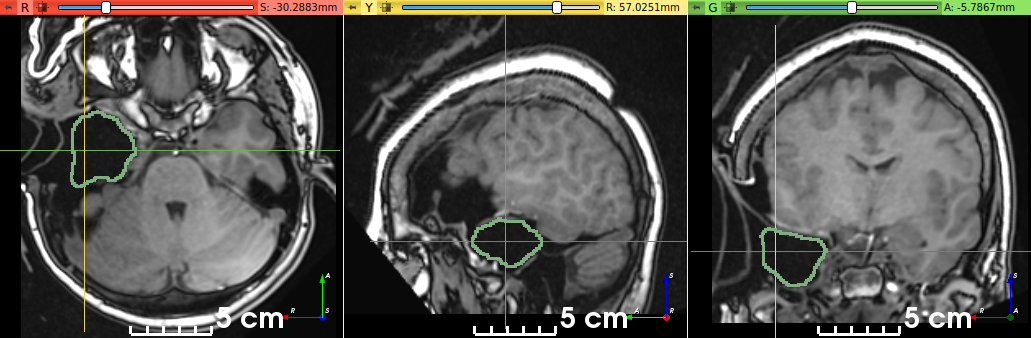
\includegraphics[trim=0 0 0 12, clip, width=\linewidth]{intra}
  \caption{
    Qualitative result on an intraoperative \ac{MRI}.
    The baseline model correctly discarded regions filled with air or \ac{CSF} outside of the \ac{RC}.
  }
  \label{fig:intra}
\end{figure}
